\section{Introducción}

En la primera instancia del curso se repasaron los conceptos básicos de Python y las librerias Numpy, Matplotlib y PySerial. En este trabajo se propuso controlar, mediante puerto serie, los parámetros del filtro Coseno Realzado (RC) y Raíz Coseno Realzado (RRC). Estos dos filtros son muy utilizados en comunicaciones digitales, y serán un concepto de utilidad en el futuro junto con la comunicación serie, cuando se diseñen filtros reales en una FPGA y esta se controle de forma remota.

\section{Desarrollo}

\subsection{Comunicación en Serie entre Dos Scripts}

En el curso se brindaron tres scripts:

\begin{itemize}
    \item \texttt{com\_serie.py}: la interfaz de comunicacion por UART.
    \item \texttt{filtro.py}: contiene la clase \textit{Filtro}, con métodos para ingresar los parámetros del RC, obtener sus coeficientes y graficarlo.
    \item \texttt{plot\_example.py}: contiene ejemplos para realizar gráficos con Matplotlib.
\end{itemize}

Los dos primeros fueron modificados para poder enviar, desde \texttt{com\_serie.py}, los parámetros para la creación de un filtro RC con \texttt{filtro.py}.

Se abrieron dos puertos virtuales con el comando en linux

\begin{lstlisting}[language=bash]
    socat -d -d PTY,raw,echo=0 PTY,raw,echo=0
\end{lstlisting}

\noindent
y se conectaron los dos script mediante estos puertos. Luego, se configuro el script de filtro para que reciba los parámetros del RC así puede generar los coeficientes. Estos parámetros son:

\begin{itemize}
    \item \textbf{Rolloff}: es el exceso de ancho de banda del filtro, entre 0 y 1 (0\% y 100\% de exceso). Este parámetro afecta el ancho de banda del canal necesario para transmitir y la complejidad en la implementación, como se verá más adelante.
    \item \textbf{Duración del filtro}: es el tiempo en símbolos que dura el filtro, se puede decir que indica la cantidad de símbolos que abarca.
    \item \textbf{Oversampling}: es la cantidad de muestras por símbolo con la que se trabaja en el filtrado.
    \item \textbf{Raíz Coseno Realzado}: es una bandera que indica si lo que se desea generar es un coseno realzado o un raíz coseno realzado.
\end{itemize}

Se desarrollaron los scripts para generar una interfaz en la que se puedan enviar los parámetros al iniciar. En la figura \ref{fig:interfaz} se observa esta interfaz, y en la figura \ref{fig:interfaz_coef} se observa cómo se reciben los coeficientes del filtro cuando se envía el comando correspondiente. El mensaje \textit{ToSent} indica que está esperando una entrada del usuario, y los mensajes que comienzan con \texttt{\textgreater\textgreater} son respuestas enviadas por el script receptor (\texttt{filtro.py} en este caso).

\begin{figure}[H]
    \centering
    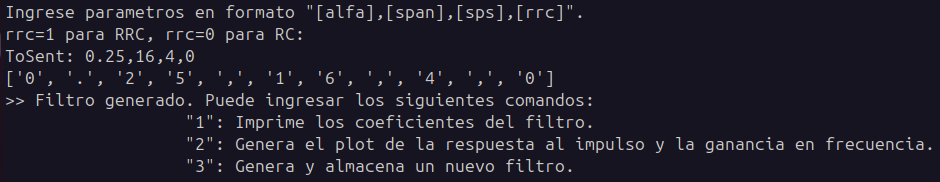
\includegraphics[width=0.85\linewidth]{img/interfaz.png}
    \caption{Interfaz de inicio.}
    \label{fig:interfaz}
\end{figure}

\begin{figure}[H]
    \centering
    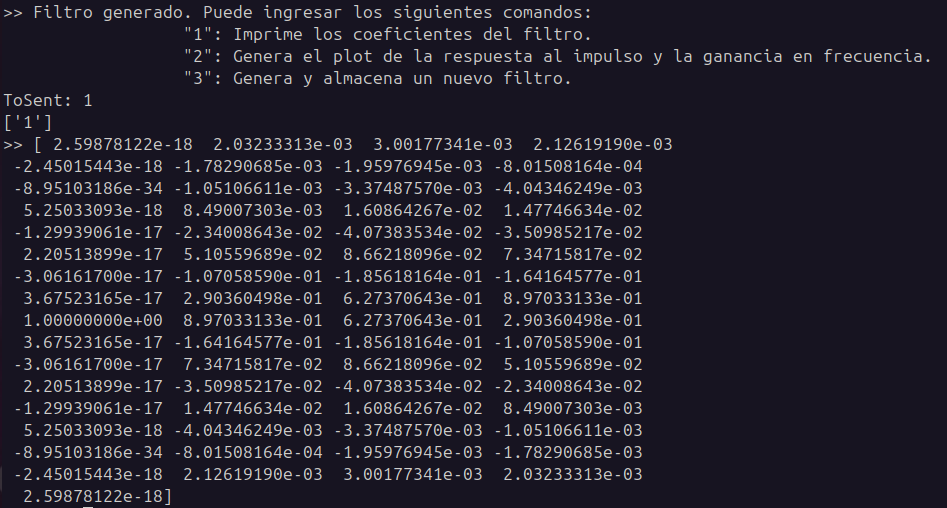
\includegraphics[width=0.85\linewidth]{img/interfaz_coef.png}
    \caption{Impresión de coeficientes del filtro generado.}
    \label{fig:interfaz_coef}
\end{figure}

\subsection{Generación y Análisis de Gráficas}

El script de Filtro original solo generaba una gráfica por filtro, entonces se lo modificó para que la clase almacene una lista de filtros con distintos parámetros, y de esta forma, graficarlos en un mismo plot. Se variaron los cuatro parámetros uno por uno, manteniendo constante los demás. Además, los plots en el tiempo se realizaron de forma discreta para representar mejor la naturaleza de un filtro digital.

En primer lugar se jugó con el rolloff y se graficaron los plots de la figura \ref{fig:rc_alpha}. En el dominio del tiempo se puede observar que un rolloff muy alto provoca que la respuesta al impulso sea más acotado, es decir, decaiga más rápido en amplitud. Y esta es una ventaja del RC, ya que en la implementación física de un FIR no se desearía tener muchos taps porque ocuparía mucha area. Sin embargo, la desventaja de un RC corto es que se extiende más en frecuencia, lo que puede generar interferencias a otros canales vecinos. Por otro lado, se observa que la frecuencia de corte de todos los filtros es de $\frac{\pi}{4}$, que es la tasa de símbolo con oversampling de 4.

Luego se varió la duración del filtro, con resultados mostrados en la figura \ref{fig:rc_span}. En el tiempo, claramente se espera ver al filtro de mayor duración por sobre las demás, sin embargo, en frecuencia se observan cambios en la atenuación, y esto es porque, con menos duración, los valores de la respuesta se cortan a cero repentinamente generando componentes de alta frecuencia.

Variando las muestras por símbolo, se obtiene lo que se ve en la figura \ref{fig:rc_sps}. Nuevamente en el tiempo se espera que el filtro con mayor sobremuestreo se superponga sobre las demás. En frecuencia, la banda de paso es mayor para los filtros con menor sobremuestreo, ya que una tasa de muestreo mayor permite abarcar mas componentes de frecuencia. Algo interesante a destacar es la diferencia de ganancia en la banda de paso, siendo de 24, 18, 12 y 6\,dB para un SPS de 16, 8, 4 y 2 respectivamente. Esto se debe a que la amplitud de las ``señales'' son iguales, pero la cantidad de muestras es distinta, resultando en una potencia diferente en cada una.

\begin{figure}[t]
    \centering

    \begin{minipage}{0.85\linewidth}
        \centering
        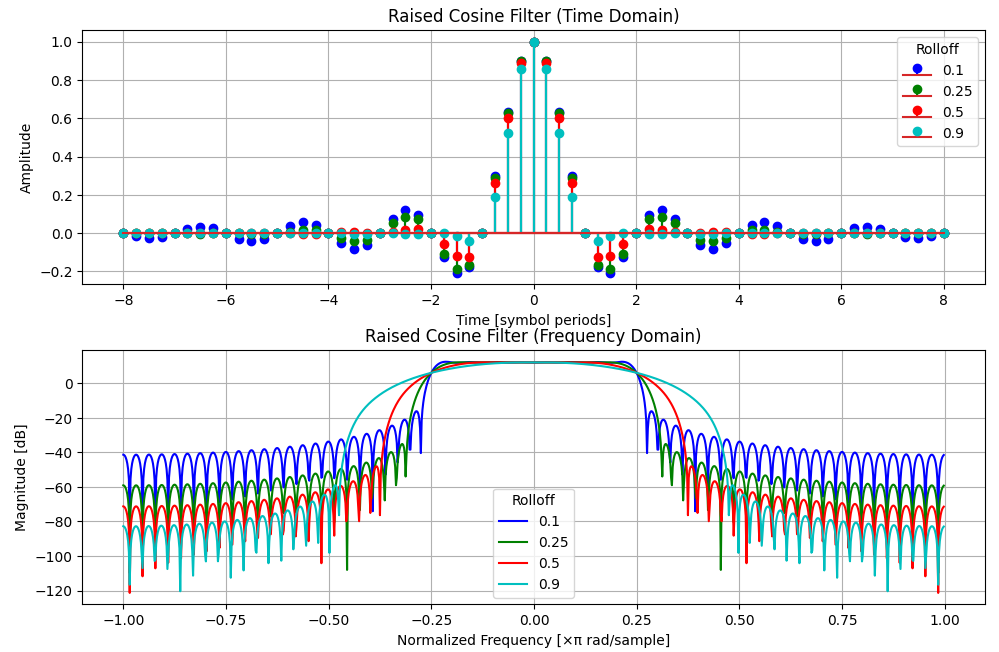
\includegraphics[width=1\linewidth]{img/rc_alpha.png}
    \end{minipage}

    \begin{minipage}{0.85\linewidth}
        \centering
        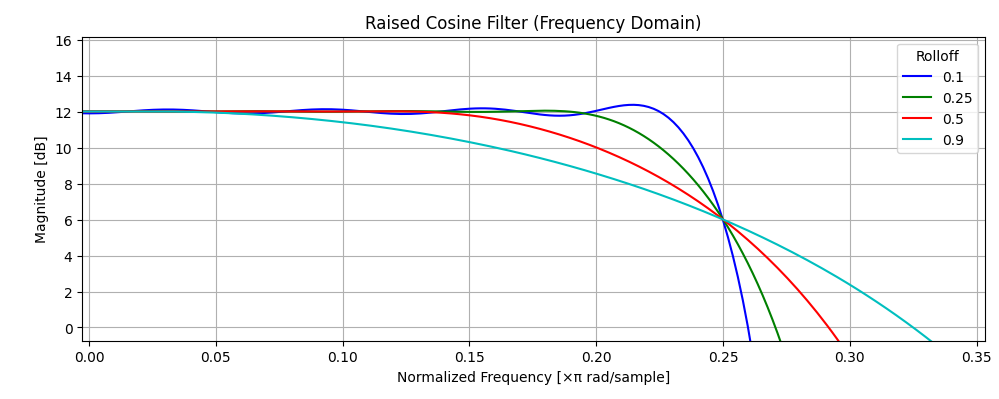
\includegraphics[width=1\linewidth]{img/rc_alpha2.png}
    \end{minipage}

    \caption{Respuesta de los filtros RC según rolloff. Duración: $16T$; SPS: $4$.}
    \label{fig:rc_alpha}
\end{figure}

Finalmente se comparó un filtro RC con uno RRC, mostrados en la figura \ref{fig:rc_rrc}. Tal como se vio en la teoría, la principal diferencia en este caso es que el RRC no cruza por cero en múltiplos de T.

\begin{figure}[H]
    \centering
        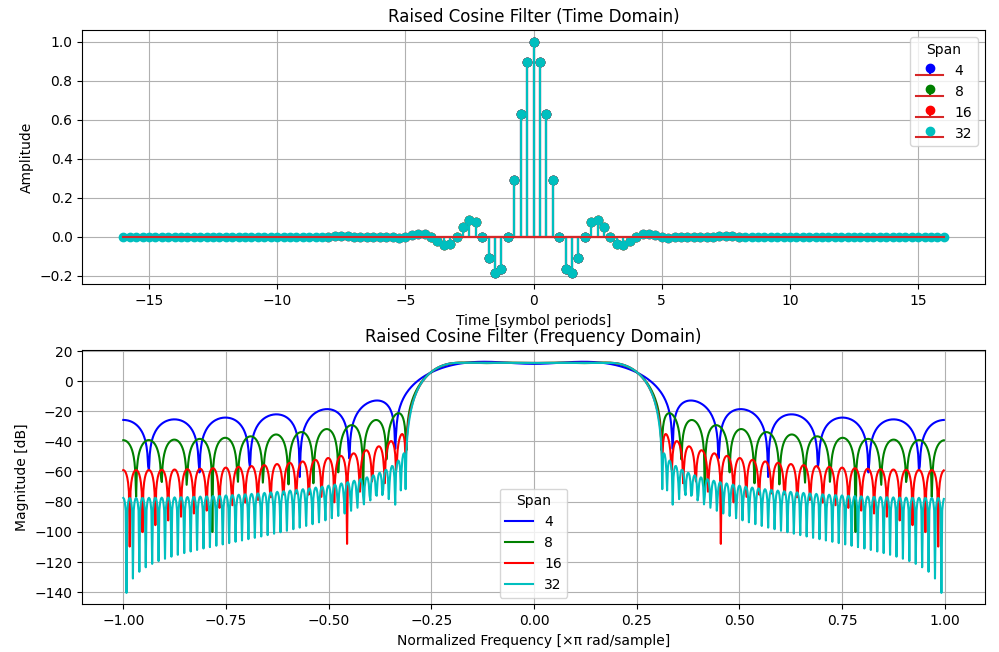
\includegraphics[width=0.75\linewidth]{img/rc_span.png}
    \caption{Respuesta de los filtros RC según su duración. Rolloff: $0.25$; SPS: 4.}
    \label{fig:rc_span}
\end{figure}

\begin{figure}[H]
    \centering

    \begin{minipage}{0.75\linewidth}
        \centering
        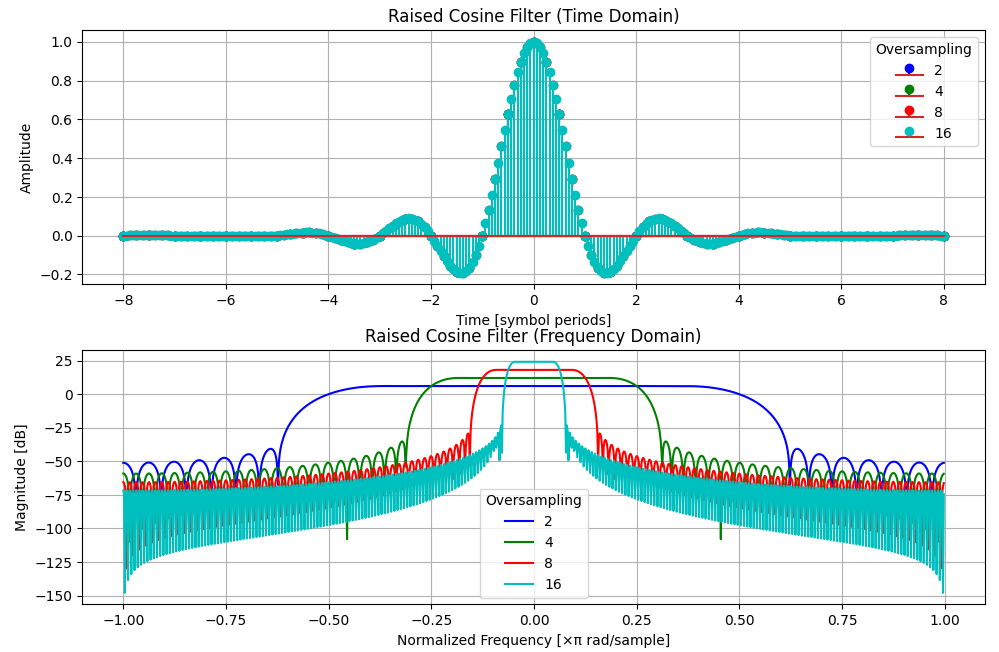
\includegraphics[width=1\linewidth]{img/rc_sps.png}
    \end{minipage}

    \begin{minipage}{0.75\linewidth}
        \centering
        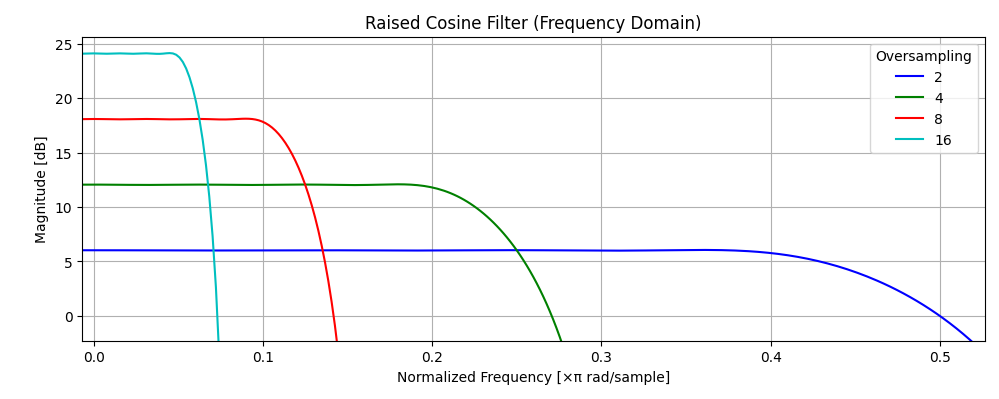
\includegraphics[width=1\linewidth]{img/rc_sps2.png}
    \end{minipage}

    \caption{Respuesta de los filtros RC según SPS. Rolloff: $0.25$; Duración: $16T$.}
    \label{fig:rc_sps}
\end{figure}

\begin{figure}[H]
    \centering
        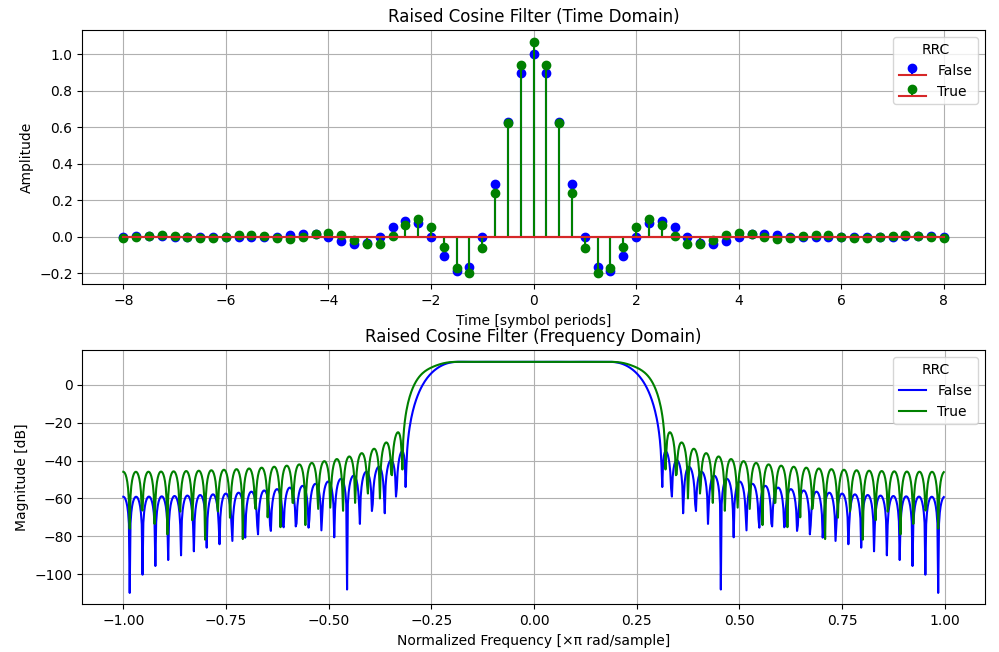
\includegraphics[width=0.85\linewidth]{img/rc_rrc.png}
    \caption{Respuesta de un RC y un RRC. Rolloff: $0.25$; Duración: $16T$; SPS: 4.}
    \label{fig:rc_rrc}
\end{figure}

\section{Conclusiones}

En este trabajo se logró realizar una comunicación por un puerto serie virtual entre dos scripts para simular el control remoto de una FPGA, algo que se necesitará hacer en trabajos futuros. Además, se exploraron distintas formas de generar gráficos, ya sea en el tiempo o frecuencia, de forma continua o discreta y con varios plots en una sola gráfica. Finalmente se analizó cómo afecta el exceso de ancho de banda, la duración y el sobremuestreo en los filtros RC y RRC.

\appendix

\section{Scripts de Python}

Los scripts \texttt{com\_serie.py} y \texttt{filtro.py} se encuentran en el siguiente link: \url{https://github.com/Ruben-Zuniga/Introduccion-al-Disenio-Digital}


% \[
%     V_{RRM} = V_{S12} = \sqrt{3} \ \hat{V}_{S} = \sqrt{3} \frac{\pi}{3\sqrt{3}} \ V_{L(AV)}
% \]

% \begin{equation}
%     \boxed{
%         V_{RRM} =  \frac{\pi}{3} \ V_{L(AV)}
%     }
% \end{equation}

% \begin{table}[H]
%     \centering
%     \begin{tblr}{
%         row{1} = {Titulo},
%         column{1} = {Titulo},
%         colspec = {Q[l] Q[c] Q[c]},
%         vlines,
%         hlines,
%         width=\linewidth
%     }
%         Parámetro & Símbolo & Valor \\
%         Máxima corriente de drenador continua ($T_C=25^\circ$C)                 & $I_{D,continua}$  & $36$ A            \\
%         Máxima tensión drenador-surtidor                                        & $V_{DSS}$         & $100$ V           \\
%         Resistencia drenador-surtidor en conducción ($V_{GS}=10$ V, $I_D=18$ A) & $R_{DS(on)}$      & $44$ m$\Omega$    \\
%         Máxima tensión puerta-surtidor                                          & $V_{GS}$          & $\pm 16$ V        \\
%         Tensión puerta-surtidor umbral                                          & $V_{GS(th)}$      & $1.4$ V           \\
%         Máxima disipación de potencia ($T_C=25^\circ$C)                         & $P_{max}$         & $140$ W           \\
%         Tiempo de retardo de encendido                                          & $t_{d(on)}$       & $11$ ns           \\
%         Tiempo de subida                                                        & $t_r$             & $81$ ns           \\
%         Tiempo de retardo de apagado                                            & $t_{d(off)}$      & $39$ ns           \\
%         Tiempo de bajada                                                        & $t_f$             & $62$ ns           \\

%     \end{tblr}
%     \caption{Parámetros característicos del IRL540.}
%     \label{tab:mosfet}
% \end{table}

% \begin{figure}[H]
%     \centering

%     \begin{minipage}{0.48\linewidth}
%         \centering
%         \includegraphics[width=1\linewidth]{img/ondas_completo1.png}
%     \end{minipage}
%     \hfill
%     \begin{minipage}{0.48\linewidth}
%         \centering
%         \includegraphics[width=1\linewidth]{img/ondas_completo2.png}
%     \end{minipage}

%     \caption{Formas de onda teóricas del convertidor.}
%     \label{fig:ondas}
% \end{figure}

% \begin{figure}[H]
%     \centering
%     \includegraphics[width=0.85\linewidth]{img/sim.png}
%     \caption{Formas de onda del rectificador hexafásico.}
%     \label{fig:sim}
% \end{figure}